\section{Method}
\label{sec:method}

\paragraph{Methodological pitfalls.}
\label{sec:pitfalls}
Lead-lag analysis in iterative model collapse is fragile along three axes, each documented with data from \S\ref{sec:regime}--\ref{sec:dose_response}.
\emph{Method sensitivity}: five detection methods applied to identical data ($\alpha{=}1.0$, 16 canary$\to$downstream pairs) yield significance rates from 100\% (naive cross-correlation) to 37.5\% (permutation Granger), with inter-method agreement at $\kappa{=}0.187$ and a spurious-signal rate ${\geq}62.5\%$.
\emph{Spurious regression}: first-differencing to remove shared trends~\cite{granger1974spurious} eliminates canary$\to$perplexity associations ($F{\approx}0$, $p{=}0.99$) while preserving canary$\to$diversity (24/24$\to$24/24), exposing an entire analysis channel as trend-driven rather than temporally precedent.
\emph{Regime dependence}: the same Granger test finds 0/8 pairs significant through $\alpha{=}0.45$ but 6/8 at $\alpha{=}0.50$, a categorical shift at a 5-percentage-point boundary that a single-$\alpha$ study would miss entirely.
These pitfalls motivate systematic method comparison rather than reliance on any single detection approach.

\paragraph{Multi-Method Consensus Test (MMCT).}
\label{sec:mmct}
We apply the Multi-Method Consensus Test, a weighted consensus framework in the specification curve~\cite{simonsohn2020specification} and multi-method early-warning~\cite{scheffer2009early,bell2022modeling} traditions, adapted to the constraints of iterative training analysis: short series ($T{=}5$--$20$), non-stationarity by design, and heterogeneous method sensitivities.
MMCT is a consensus testing protocol, not a novel statistical method.
It compares five lead-lag detection methods through FPR-inverse weighted consensus, calibrated against null-control ($\alpha{=}0.0$) data where any detection is a false positive.
Each method $m_k$ receives weight $w_k = 1/\max(\hat{\text{FPR}}_k, \epsilon)$ with $\epsilon{=}0.01$; the weighted score $W(X \to Y) = \sum_k w_k d_k / \sum_k w_k$ yields formal $p$-values from the empirical null distribution (Algorithm~\ref{alg:mmct}; Appendix).
MMCT identifies permutation Granger (PermG) as the method with the lowest null-control FPR among directionally-specific methods (11.1\%, 4/36 across 6 seeds; DiffXCorr achieves 2.8\% but lacks directional separation) combined with consistent detection across contamination levels, and we recommend it as the primary detection method based on this systematic comparison.

\paragraph{Permutation Granger causality.}
PermG tests whether past values of canary metric $X$ improve prediction of downstream metric $Y$ beyond $Y$'s own history; Granger precedence establishes temporal predictive improvement, not true causality~\cite{shojaie2022granger}.
We apply 5{,}000 permutations on first-differenced series with Benjamini--Hochberg FDR correction at $q{=}0.05$ across 8 validated canary$\to$downstream pairs (2 canaries $\times$ 4 downstream metrics).
Three properties distinguish PermG: a nonparametric null distribution robust to the short non-stationary series typical of iterative training~\cite{boettiger2012limits}, built-in directionality (forward and reverse tested separately), and a hyperparameter-free test statistic.
The remaining four methods each exhibit a specific limitation: naive cross-correlation has 75\% null-control FPR; differenced cross-correlation detects bidirectionally without directional separation; threshold onset is power-limited at $T{=}11$ under corrected $3\sigma$ calibration (0/8 significant in 8 of 12 cross-architecture conditions); Toda--Yamamoto~\cite{toda1995statistical} achieves moderate supplementary detection (3--4/8 at $\alpha{\geq}0.50$) with reduced power from degree-of-freedom costs of lag augmentation.
Per-method dose-response profiles, Shapley value analysis, and the full MMCT algorithm appear in the Appendix.

\begin{figure*}[t]
\centering
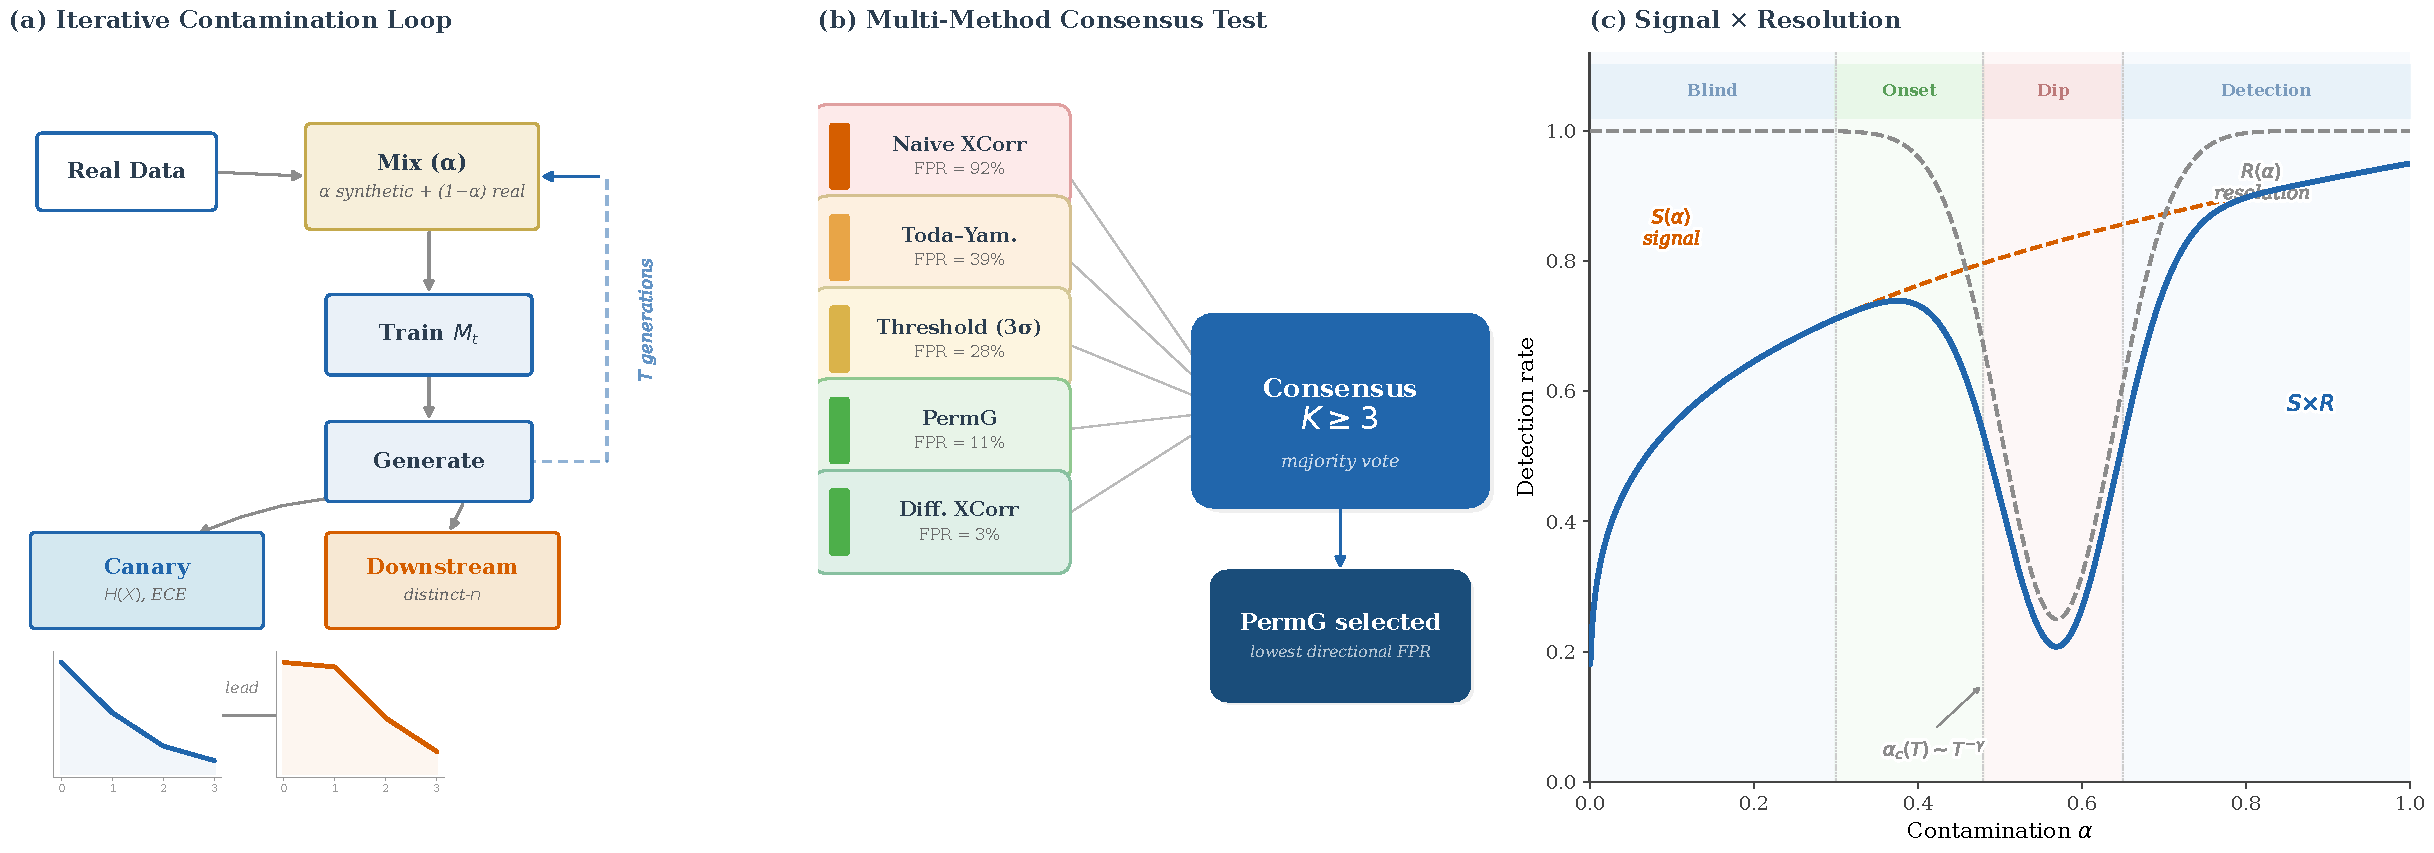
\includegraphics[width=\textwidth]{figures/fig_framework.pdf}
\caption{Analytical framework overview. (a)~Iterative contamination loop: each generation fine-tunes on an $\alpha$-fraction synthetic mixture, producing canary (entropy, ECE) and downstream (distinct-$n$, perplexity) time series. (b)~Multi-Method Consensus Test: five detection methods weighted by inverse null-control FPR converge to a $K{\geq}3$ consensus decision. (c)~Detection regimes in the $(\alpha, T)$ plane: the boundary $\alpha_c(T)$ separates blind and detection zones, with onset and sync-dip as transitional regions.}
\label{fig:framework}
\end{figure*}

\subsection{Signal-Times-Resolution Framework}
\label{sec:theory}

We apply standard statistical power scaling to PermG under the Signal$\times$Resolution (S$\times$R) framework.
Detectability of canary$\to$downstream temporal precedence depends on two competing factors:
\begin{equation}
    \text{Detectability}(\alpha) \;\propto\; S(\alpha) \times R(\alpha),
    \label{eq:detectability}
\end{equation}
where $S(\alpha)$ is signal strength (magnitude of distributional shift, monotonically increasing with $\alpha$) and $R(\alpha)$ is temporal resolution (the generational gap between canary and downstream responses).
$R(\alpha)$ is non-monotonic: at low $\alpha$, entropy and diversity respond in different generations ($R$ large); at $\alpha{\approx}0.60$, relaxation time matching compresses both responses into a single generation ($R \to 0$); at high $\alpha$, the severity of entropy collapse outpaces the diversity cascade, restoring the generational offset.
The product $S \times R$ predicts four regimes: \emph{blind} ($\alpha \leq 0.45$; $S$ below detection floor), \emph{onset} ($\alpha \approx 0.50$; $S$ crosses threshold while $R$ remains high), \emph{synchronous dip} ($\alpha \approx 0.60$; $R \to 0$ suppresses detection despite rising $S$), and \emph{detection} ($\alpha \geq 0.75$; $S$ dominates).
Full empirical confirmation appears in \S\ref{sec:regime} and \S\ref{sec:dose_response}.

Under a permutation test framework, detection power scales as $\mathrm{Power}(\alpha, T) = \Phi\bigl(S \cdot R \cdot \sqrt{T} / \sigma_{\mathrm{noise}}\bigr)$, where $\Phi$ is the standard normal CDF and the $\sqrt{T}$ scaling follows standard power analysis.
The sharp detection onset at $\alpha_c$ (at $T{=}10$) is consistent with a power threshold: when $S \cdot R \cdot \sqrt{T}$ first exceeds the detection floor, power undergoes a steep onset from near-zero to near-one.
This generates three predictions for $T{=}20$: (i)~$\alpha_c$ left-shifts as increased $T$ raises power at all $\alpha$; (ii)~the transition smooths as $\sqrt{T}$ broadens the power curve; (iii)~different methods exhibit different $\alpha_c$ values due to method-specific power curves.
Bootstrap calibration ($N{=}10{,}000$) yields clean falsifiable tests at $\alpha{\geq}0.75$: predicted 7/8 (95\% CI: [6,8]); results below 6/8 would falsify $\sqrt{T}$ power scaling.
At $\alpha{=}0.45$, the point prediction is 0/8, but the bootstrap CI spans [0,7] reflecting $\alpha_c$ uncertainty---both detection and non-detection are informative for constraining the phase boundary location.
At $\alpha{=}0.50$, the prediction is inherently uncertain at the transition (CI: [0,7]).
Sub-threshold FDR $p{=}0.059$--$0.091$ at $\alpha{=}0.45$ is consistent with proximity to the power boundary.

\paragraph{Calibration.}
We validate error rates with built-in experimental controls.
False positive rate: at $\alpha{=}0.0$ (null control, no synthetic contamination), PermG achieves the lowest FPR among directionally-specific methods: 11.1\% across 6 seeds (4/36 pairs; Clopper--Pearson 95\% CI $[3.1\%, 26.1\%]$); under identical BH-FDR correction, DiffXCorr achieves the lowest FPR (2.8\%) but lacks forward/reverse directional separation.
False negative rate: at $\alpha{=}1.0$, all 6 effect-size reference pairs (2 canaries $\times$ 3 diversity metrics, selected by criteria independent of the detection methods) are recovered at 0\% FNR across 4 seeds.
PermG matches consensus performance at all tested contamination levels, with cross-architecture validation confirming PermG forward significance ${\geq}6/8$ in 11 of 15 conditions (\S\ref{sec:generalization}).
Full calibration details, practical guidance tiers, and method-level breakdown appear in the Appendix.
